\documentclass[preview]{standalone}

\usepackage{amsmath}
\usepackage{amssymb}
\usepackage{stellar}
\usepackage{chemfig}

\hypersetup{
    colorlinks=true,
    linkcolor=black,
    urlcolor=blue,
    pdftitle={Stellar},
    pdfpagemode=FullScreen,
}

\begin{document}

\title{Stellar}
\id{chimica-idrocarburi}
\genpage

\section{Idrocarburi}

\begin{snippetdefinition}{Idrocarburi-definizione}{Idrocarburi}
    Gli \textit{idrocarburi} sono costituiti esclusivamente da atomi di
    carbonio e idrogeno.
\end{snippetdefinition}

\begin{snippetdefinition}{alcani-definizione}{Alcani}
    Gli \textit{alcani} sono composti idrocarburi saturi, in cui sono presenti solo
    legami singoli quelli a catena aperta hanno formula generale
    C\({}_n\)H\({}_{2n+2}\) dove n indica il numero di atomi di carbonio.
\end{snippetdefinition}

\begin{snippet}{punto-ebollizione-alcani}
    Il punto di ebollizione degli alcani aumenta progressivamente con
    l'aumentare della massa molecolare, perché le forze di London
    diventano sempre più intense. Sono in genere meno densi
    dell'acqua.
\end{snippet}

\begin{snippetdefinition}{alcheni-definizione}{Alcheni}
    Gli \textit{alcheni} sono idrocarburi che contengono uno o più doppi
    legami carbonio-carbonio.
    Quelli a catena aperta hanno formula generale, C\({}_n\)H\({}_{2n}\)
    dove n indica il numero di atomi di carbonio.
\end{snippetdefinition}

\begin{snippetdefinition}{alchini-definizione}{Alchini}
    Gli \textit{alchini} sono idrocarburi che presentano un triplo legame. Quelli a catena
    aperta hanno formula generale C\({}_n\)H\({}_{2n-2}\)
    dove n indica il numero di atomi di carbonio.. 
\end{snippetdefinition}

\plain{Gli alchini sono insolubili in acqua e sono facilmente infiammabili.}

\section{Isomeria geometrica negli Alcheni}

\begin{snippet}{regole-isomeria-alcheni}
    \begin{itemize}
        \item Gli alcheni possono mostrare un \textit{isomeria geometrica} con una diversa direzione dei gruppi
        legati al doppio legame
        \item Quando i due sostituenti sono dalla stessa parte si parla di \textbf{isomero cis} mentre quando
        puntano in direzione opposta di \textbf{isomero trans}.
    \end{itemize}
\end{snippet}

\begin{snippet}{trans-cis-isomero-illustration}
    \begin{center}
    \begin{figure}
        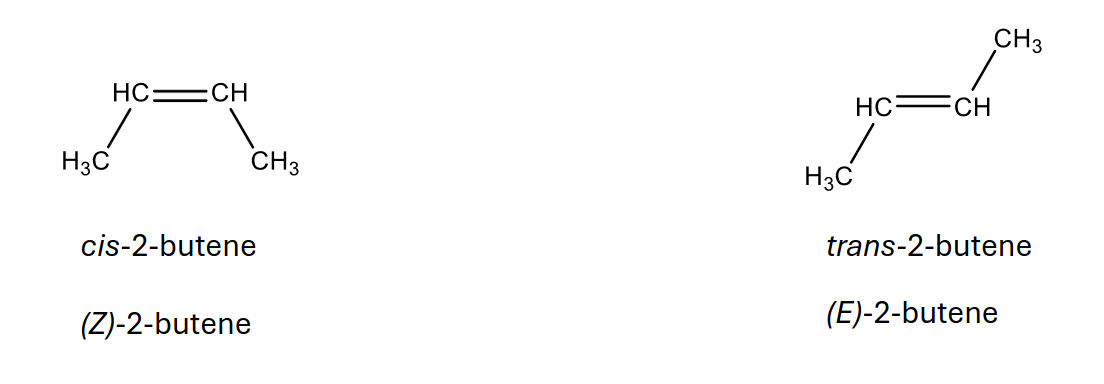
\includegraphics[width=0.75\textwidth]{./resources/trans_cis_isomero.png}
    \end{figure}
    \end{center}
\end{snippet}

\section{Nomenclatura sistematica degli alcani}

% Il 2-butatone si puô anche scrivere senza il 2, perché è l'unica possibilità
% Nel disegno della formula i legami tripli sono sempre lineari.


\end{document}